\section{Theory}
\paragraph{Gamma radiation?}

\paragraph{Scintillation detector}
Scintillation detectors are based on the properties of \emph{scintillators}, materials that emit photons in the visible spectrum after the passage of a charged particle.
The scintillators used for particle detection are primarily [split] between two types: organic (or plastic), in which the photon emission has molecular origin, 
and inorganic (or crystalline), crystals which are doped with activators that can first be excited by electron-hole pairs 
produced by the charged particle passing in the crystal lattice\footnotemark and then de-excited by photon emission\cite{intro_nuclear_particle_physics}.
Because of the low intensity of the emitted light, the photon signal must be amplified in order to be properly counted.
This amplification is commonly achieved through the use of photomultiplier tubes (PMT), a device which converts the photon signal in a detectable electric pulse.
It consists of a vacuum tube [chamber?] containing several components, pictured in Fig. \ref{fig:photomultiplier}: 
after passing a transparent entry window, adjacent to the scintillator, the scintillation photons first encounter a photocatode, 
where they produce an electron by photoelectric effect with a certain probability $\varepsilon$ (the quantum efficacy).
Next, a series of dynodes accellerate the electrons and multiply them thorugh secondary emission
\footnotetext{Ici je pourrai écrire "produced by the passing charged particle" sans specifier, pour rendre la phrase un peu plus legere.}
\begin{figure}[htbp]
    \centering
    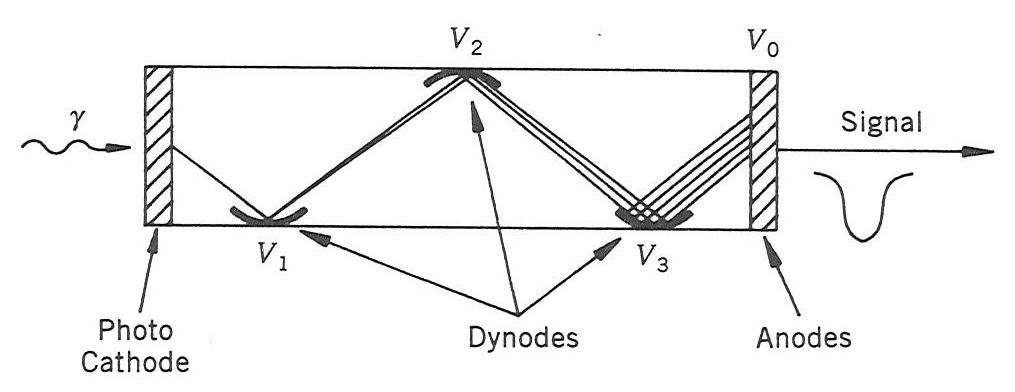
\includegraphics[scale=1]{figures/photomultiplier.jpg}
    \caption{Main elements of a photomultiplier tube \cite{intro_nuclear_particle_physics}.}
    \label{fig:photomultiplier}
\end{figure}

\paragraph{Gamma spectrometry}
Page 144 de \cite{intro_nuclear_particle_physics} pour expliquer les effets de l'effet compton
[Expliquer l'apparition d'une gaussienne à la place d'une ligne pour les peaks des spectres]


\paragraph{Experimental setup}
[? dire que on utilise inorganic?]